\documentclass{article}
\usepackage[utf8]{inputenc}
\usepackage[T1]{fontenc}
\usepackage[utf8]{inputenc}
\usepackage[norsk]{babel}
\usepackage{amsmath}
\usepackage{verbatim}
\usepackage{hyperref}
\usepackage{enumerate}
\usepackage{graphicx}
\usepackage{listings}
\usepackage{color}
\usepackage{gensymb}
\usepackage{subfig}
\usepackage{fancyvrb}
\definecolor{codegreen}{rgb}{0,0.6,0}
\definecolor{codegray}{rgb}{0.5,0.5,0.5}
\definecolor{codepurple}{rgb}{0.58,0,0.82}
\definecolor{backcolour}{rgb}{0.95,0.95,0.92}
\setlength{\parindent}{0pt}
\lstdefinestyle{mystyle}{
    backgroundcolor=\color{backcolour},
    commentstyle=\color{codegreen},
    keywordstyle=\color{magenta},
    numberstyle=\tiny\color{codegray},
    stringstyle=\color{codepurple},
    basicstyle=\footnotesize,
    breakatwhitespace=false,
    breaklines=true,
    captionpos=b,
    keepspaces=true,
    numbers=left,
    numbersep=5pt,
    showspaces=false,
    showstringspaces=false,
    showtabs=false,
tabsize=2}
\lstset{style=mystyle}

\title{Ukesoppgaver inf4470}
\author{mathiaki}


\begin{document}

\maketitle

\newpage
\tableofcontents
\newpage

\section{Appendix A}
\lstinputlisting[language=Matlab]{uke10.m}
\newpage
\newpage
\section{Oppgave 1}
\subsection{hamming}
\begin{figure}[h]%
		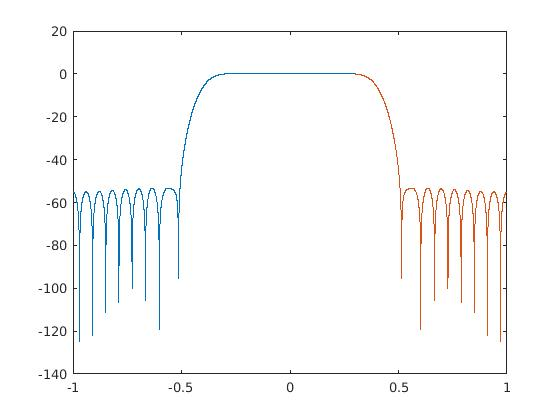
\includegraphics[scale=0.50]{oppg1hamming1.jpg}
	    \caption{oppg1}
    	\label{fig:otsuandfriends}%
\end{figure}	

\begin{figure}[h]%
		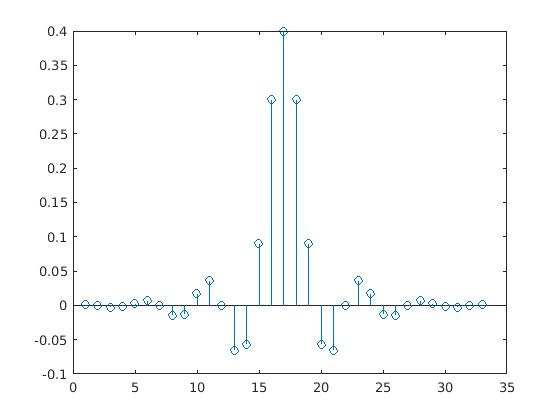
\includegraphics[scale=0.5]{oppg1hamming2.jpg}
	    \caption{oppg1}
    	\label{fig:otsuandfriends}%
\end{figure}	


\begin{figure}[h]%
		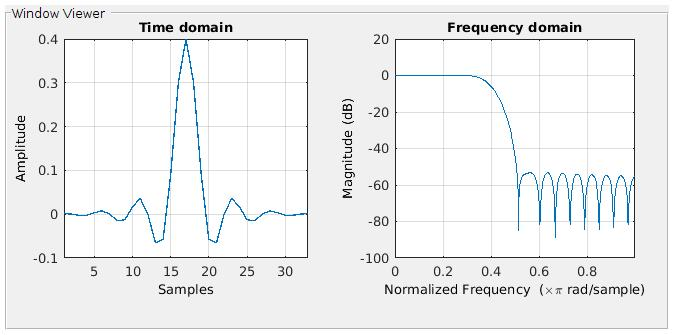
\includegraphics[scale=0.5]{oppg1hamming3.jpg}
	    \caption{oppg1}
    	\label{fig:otsuandfriends}%
\end{figure}		 
\newpage
\newpage
\newpage
\newpage
\subsection{Kaiser}

\begin{figure}[h]%
		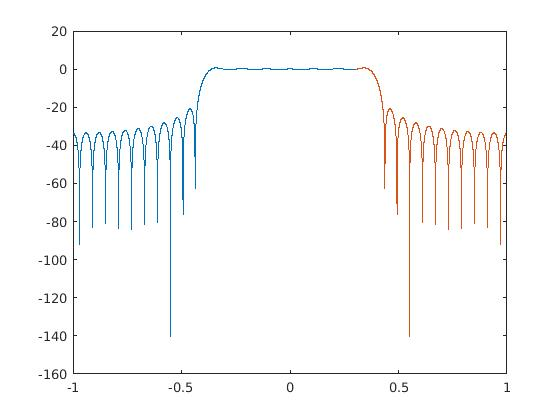
\includegraphics[scale=0.5]{oppg1kaiser1.jpg}
	    \caption{oppg1}
    	\label{fig:otsuandfriends}%
\end{figure}	

\begin{figure}[h]%
		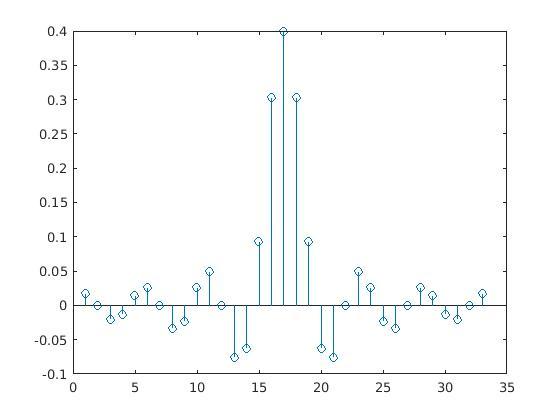
\includegraphics[scale=0.5]{oppg1kaiser2.jpg}
	    \caption{oppg1}
    	\label{fig:otsuandfriends}%
\end{figure}	


\begin{figure}[h]%
		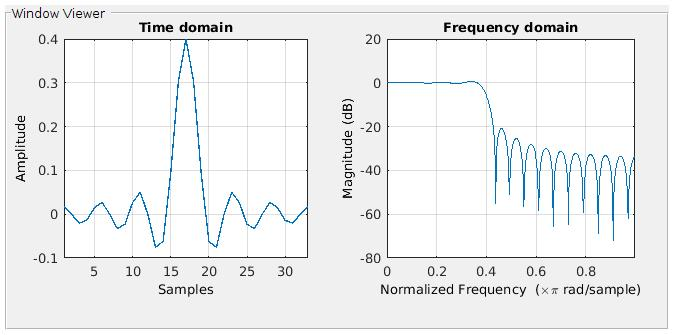
\includegraphics[scale=0.5]{oppg1kaiser3.jpg}
	    \caption{oppg1}
    	\label{fig:otsuandfriends}%
\end{figure}
\newpage
\newpage
\newpage
\newpage


\section{Oppgave 2}

\begin{figure}[h]%
		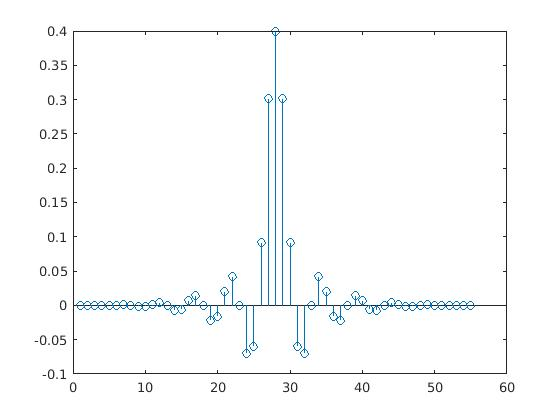
\includegraphics[scale=0.5]{oppg2.jpg}
	    \caption{oppg2}
    	\label{fig:otsuandfriends}%
\end{figure}	

\begin{figure}[h]%
		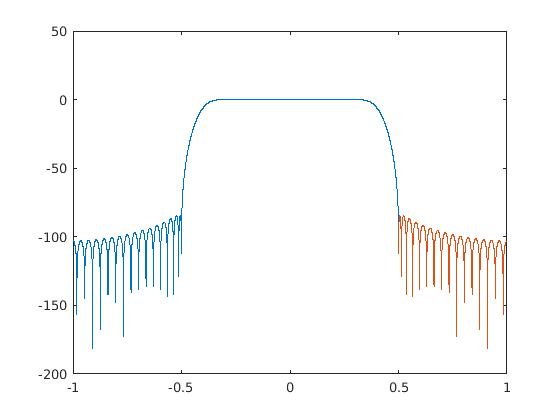
\includegraphics[scale=0.5]{oppg2_1.jpg}
	    \caption{oppg2}
    	\label{fig:otsuandfriends}%
\end{figure}	


\begin{figure}[h]%
		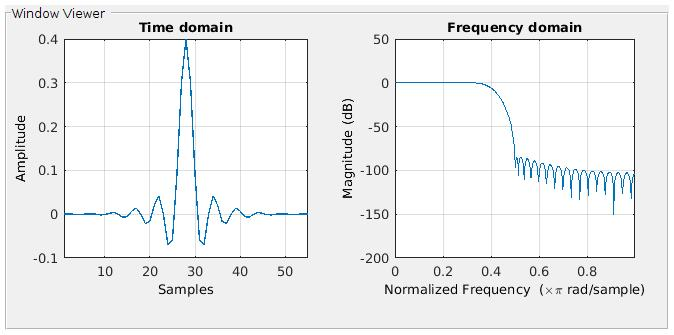
\includegraphics[scale=0.5]{oppg2_2.jpg}
	    \caption{oppg2}
    	\label{fig:otsuandfriends}%
\end{figure}
\newpage
\newpage
\newpage
\newpage
\section{Oppgave 3}



\begin{figure}[h]%
		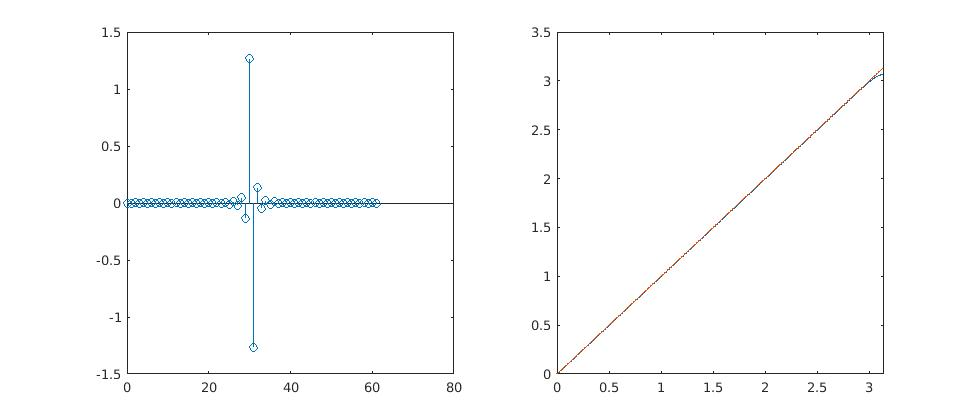
\includegraphics[scale=0.5]{oppg3.jpg}
	    \caption{oppg3}
    	\label{fig:otsuandfriends}%
\end{figure}	

\begin{figure}[h]%
		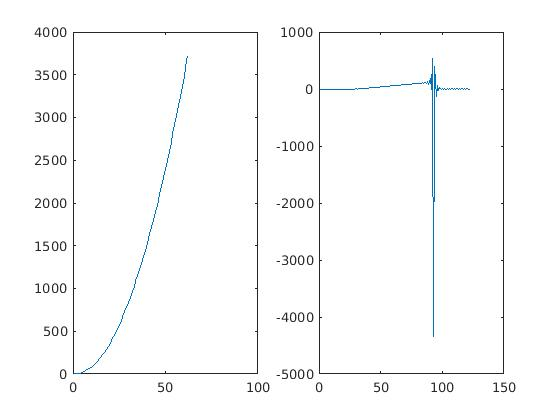
\includegraphics[scale=0.5]{oppg31.jpg}
	    \caption{oppg3}
    	\label{fig:otsuandfriends}%
\end{figure}	


\begin{figure}[h]%
		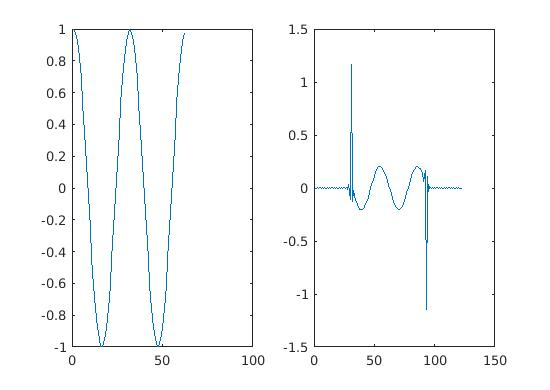
\includegraphics[scale=0.5]{oppg32.jpg}
	    \caption{oppg3}
    	\label{fig:otsuandfriends}%
\end{figure}

\begin{figure}[h]%
		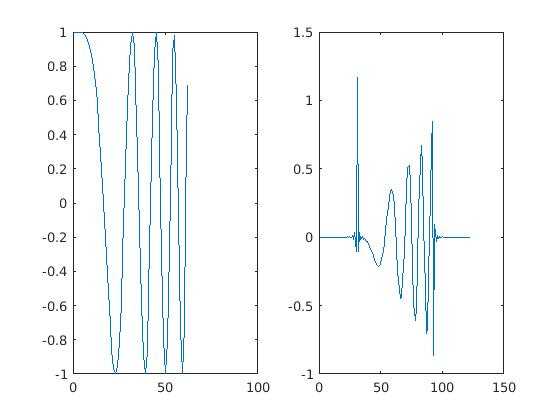
\includegraphics[scale=0.5]{oppg33.jpg}
	    \caption{oppg3}
    	\label{fig:otsuandfriends}%
\end{figure}
\newpage
\newpage
\newpage
\newpage
\newpage



\section{Oppgave 4}
\begin{figure}[h]%
		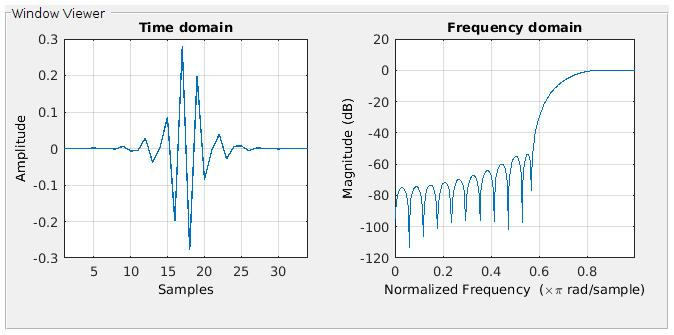
\includegraphics[scale=0.5]{oppg4.jpg}
	    \caption{oppg4}
    	\label{fig:otsuandfriends}%
\end{figure}

\begin{figure}[h]%
		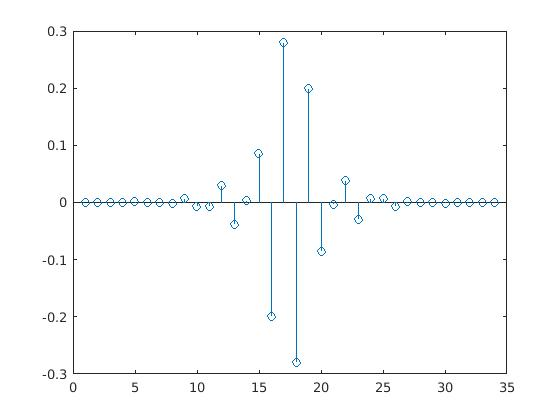
\includegraphics[scale=0.5]{oppg41.jpg}
	    \caption{oppg4}
    	\label{fig:otsuandfriends}%
\end{figure}



\end{document}\\

